% override specific chktex warnings

% chktex-file 1 - ignore commands followed by a space, e.g. \\ new line here
% chktex-file 3 - enclose previous parentheses wit {}
% chktex-file 9 - sometimes messes up with ( and {
% chktex-file 36 - put a space in front of parentheses
% chktex-file 45 - don't use $$ instead of \[, etc
% chktex-file 46 - don't use $ instead of \(, etc


\documentclass[10pt, oneside]{amsart}
% \usepackage[showboxes]{textpos}

\usepackage[absolute,overlay]{textpos}
\setlength{\TPHorizModule}{1.0cm}
\setlength{\TPVertModule}{\TPHorizModule}
\textblockorigin{0.0cm}{0.0cm}  %start all at upper left corner

\usepackage{amsmath}
\usepackage{amsthm}
\usepackage{amsfonts}
\usepackage{amssymb}
\usepackage{mathpazo}
\usepackage{booktabs}
\usepackage[usenames,x11names]{xcolor}
\usepackage{tikz}
\usepackage{textcomp}
\usepackage[letterpaper]{geometry}
\geometry{verbose,tmargin=0.5in,bmargin=0.5in,lmargin=1in,rmargin=0.5in}
\usepackage{multicol}
\usepackage{bm}
\usepackage{comment}
\usepackage{cancel}
\usepackage{array}
\usepackage{gensymb}
\usepackage{enumerate}
\usepackage[many]{tcolorbox}

\pagestyle{plain}
\raggedright
\renewcommand{\familydefault}{\sfdefault}
\setlength{\parskip}{\medskipamount}
\setlength{\columnsep}{1cm}

\everymath{\displaystyle}
\setlength{\parskip}{\bigskipamount}

% counter for resuming enumerated list numbers
\newcounter{resumeenumi}
\newcommand{\suspend}{\setcounter{resumeenumi}{\theenumi}}
\newcommand{\resume}{\setcounter{enumi}{\theresumeenumi}}

\newcommand\lb{\linebreak}
\newcommand\pars{\par\smallskip}
\newcommand\parm{\par\medskip}
\newcommand\parb{\par\bigskip}

\makeatletter
\providecommand{\gettikzxy}[3]{%
	\tikz@scan@one@point\pgfutil@firstofone#1\relax
	\edef#2{\the\pgf@x}%
	\edef#3{\the\pgf@y}%
}
\makeatother



% full width colored block but color specifiable
%\cb[body bg strength]{header bg}{header text}{body text}
\newcommand{\cb}[4][15]{
	\setbeamercolor{block title}{bg = #2}
	\setbeamercolor{block body}{bg = #2!#1}
	\setbeamercolor{item projected}{bg=#2, fg=white}
	\begin{center}
		\begin{block}{#3}
			#4
		\end{block}
	\end{center}
}

% colored block with width specified
% \cbw[body bg strength]{header bg}{width}{header text}{body text}
\newcommand{\cbw}[5][15]{
	\begin{center}
		%\vspace{-0.35cm}
		\begin{minipage}{#3\textwidth}
			\setbeamercolor{block title}{bg= #2}
			\setbeamercolor{block body}{bg= #2!#1}
			\setbeamercolor{item projected}{bg=#2, fg=white}
			\begin{block}{#4}
				\raggedright
				#5
			\end{block}
		\end{minipage}
	\end{center}
}

% centered minipage with text \raggedright
%\cmini[width]{content}
\newcommand{\cmini}[2][0.8]{
	\begin{center}
		\begin{minipage}{#1\columnwidth}
			\raggedright
			#2
		\end{minipage}
	\end{center}
}

%left flushed minipage
\newcommand{\mini}[2][0.8]{
	\begin{minipage}{#1\columnwidth}
		\raggedright
		#2
	\end{minipage}
}

%left flushed minipage, top aligned
\newcommand{\minit}[2][0.8]{
	\begin{minipage}[t]{#1\columnwidth}
		\raggedright
		#2
	\end{minipage}
}

%left flushed minipage
% \newcommand{\miniT}[2][0.8]{
%  \begin{minipage}[T]{#1\columnwidth}
%   \raggedright
%   #2
%  \end{minipage}
% }

%left flushed minipage
\newcommand{\minib}[2][0.8]{
	\begin{minipage}[b]{#1\columnwidth}
		\raggedright
		#2
	\end{minipage}
}

\newcommand{\cfig}[2][1]{% centred, scaled graphic
	\begin{center}
		\includegraphics[scale=#1]{#2}
	\end{center}
}
% figure with tight border for photos
% \cfigb[saitMaroon]{borderwidth with unit}{scale}{image}
\newcommand{\cfigb}[4][structure]{
	% \usepackage{adjustbox}
	\setlength{\fboxrule}{1pt}
	\begin{center}
		\includegraphics[scale=#3, cframe= #1 #2]{#4}
	\end{center}
}

\newcommand{\imgbox}[3]{
	% \setlength{\fboxsep}{12pt}
	\includegraphics[scale=#1, cframe= structure #3]{#2}
}

% \imgboxbg[bg color=white]{scale}{path/to/img}{border color}{border, e.g. 2pt}{margin, e.g. 4pt}
\newcommand{\imgboxbg}[6][white]{
	\setlength{\fboxrule}{#5}
	\setlength{\fboxsep}{#6}
	\centering
	\fcolorbox{#4}{#1}{\includegraphics[scale=#2]{#3}}
}

\newcommand{\fig}[2][1]{% scaled graphic
	\includegraphics[scale=#1]{#2}
}

% centred framed  box black border
%\cbox[width]{content}
\newcommand{\cbox}[2][0.9]{% framed centered  box
	\setlength\fboxsep{0.042\columnwidth}
	\setlength\fboxrule{0.0015\columnwidth}
	\begin{center}
		\fcolorbox{black}{white}{
			\vspace{-0.5cm}
			\begin{minipage}{#1\columnwidth}
				\raggedright
				#2
			\end{minipage}
		}
	\end{center}
	\setlength\fboxsep{0cm}
}



\newtcolorbox{mybox}[1][]
{
	colback=white,
	top=0.25cm,
	bottom=0.25cm,
	left=0.25cm,
	right=0.25cm,
	colframe=structure,
	fonttitle=\bfseries,
	enhanced, drop fuzzy shadow,
	% attach boxed title to top left={yshift=-2mm, xshift=5mm},
	attach boxed title to top left={yshift=-2mm, xshift=5mm}, colbacktitle=structure!80!white, #1}

\newtcolorbox{plainbox}[1][]{colback=white, sharp corners, top=0.125cm, bottom=0.125cm, left=0pt, right=0pt, boxrule=0.5pt,colframe=structure,fonttitle=\bfseries, colbacktitle=structure, arc=0mm, #1}
%
\newtcbtheorem{myexam}{Example}%
{
	enhanced,
	colback=white,
	top=0.375cm,
	bottom=0.25cm,
	left=0.375cm,
	right=0.375cm,
	colframe=structure,
	fonttitle=\bfseries,
	drop fuzzy shadow,
	%description font=\mdseries\itshape,
	attach boxed title to top left={yshift=-2mm, xshift=5mm},
	colbacktitle=structure!80!white
	}{exam}% then \pageref{exer:theoexample} references the theo

\newcommand{\myexample}[2][red]{
	% \tcb\tcbset{theostyle/.style={colframe=red,colbacktitle=yellow}}
	\begin{myexam}{}{}
		\raggedright
		#2
	\end{myexam}
	% \tcbset{colframe=structure,colbacktitle=structure}
}

\newtcbtheorem{myexer}{Exercise}%
{
	enhanced,
	colback=white,
	top=0.375cm,
	bottom=0.25cm,
	left=0.375cm,
	right=0.375cm,
	colframe=structure,
	fonttitle=\bfseries,
	drop fuzzy shadow,
	%description font=\mdseries\itshape,
	attach boxed title to top left={yshift=-2mm, xshift=5mm},
	colbacktitle=structure!80!white
	}{exer}

\newcommand{\myexercise}[2][red]{
	% \tcb\tcbset{theostyle/.style={colframe=red,colbacktitle=yellow}}
	\begin{myexer}{}{}
		\raggedright
		#2
	\end{myexer}
	% \tcbset{colframe=structure,colbacktitle=structure}
}


\begin{document}

\thispagestyle{empty}
\vspace{-7cm}
\centering
\textbf{\Large Module 8: Hazen Williams Equation and Equivalent Pipes (CIVL 318)}
\par\medskip
\centering
\cbox[0.8]{
	\centering
	\textbf{\large Hazen-Williams Equations}
	\[
		Q = \frac{C\,D^{2.63}\left(\frac{h_L}{L}\right)^{0.54}}{279000},\qquad
		h_L = L\,\left(\frac{279000\,Q}{C\,D^{2.63}}\right)^{1.852},\qquad
		D = \left(\frac{279000\,Q}{C\,\left(\frac{h_L}{L}\right)^{0.54}}\right)^{0.3802}
	\]
}
\cbox[0.7]{
	\centering
	\textbf{\Large Equivalent-Length Ratios for Fittings}
	\parb
	\begin{tabular}{r >{$}r<{$} >{$}l<{$} >{$}c<{$} }
		\toprule
		\text{Type}                                                    & \quad & L_e/D \\
		\midrule
		\addlinespace
		Globe valve --- fully open                                     &       & 340   \\
		\addlinespace
		Angle valve --- fully open                                     &       & 150   \\
		\addlinespace
		Gate valve --- fully open                                      &       & 8     \\
		\addlinespace
		--- $3/4$ open                                                 &       & 35    \\
		\addlinespace
		--- $1/2$ open                                                 &       & 160   \\
		\addlinespace
		--- $1/4$ open                                                 &       & 900   \\
		\addlinespace
		Check valve --- swing type                                     &       & 100   \\
		\addlinespace
		Check valve --- ball type                                      &       & 150   \\
		\addlinespace
		Butterfly valve --- fully open --- 2-8''                       &       & 45    \\
		\addlinespace
		--- 10-14''                                                    &       & 35    \\
		\addlinespace
		--- 16-24''                                                    &       & 25    \\
		\addlinespace
		Foot valve --- poppet disc type                                &       & 420   \\
		\addlinespace
		Foot valve --- hinged disc type                                &       & 75    \\
		\addlinespace
		$90\degree$ standard elbow                                     &       & 30    \\
		\addlinespace
		$90\degree$ long radius elbow                                  &       & 20    \\
		\addlinespace
		$90\degree$ street elbow                                       &       & 50    \\
		\addlinespace
		$45\degree$ standard elbow                                     &       & 16    \\
		\addlinespace
		$45\degree$ street elbow                                       &       & 26    \\
		\addlinespace
		Close return bend                                              &       & 50    \\
		\addlinespace
		Standard tee --- flow through run                              &       & 20    \\
		\addlinespace
		Standard tee --- flow through branch                           &       & 60    \\
		\addlinespace
		Gradual enlargement --- $15^\circ$ cone angle                  &       & 8     \\
		\addlinespace
		Gradual enlargement --- $20^\circ$ cone angle                  &       & 15    \\
		\addlinespace
		Gradual enlargement --- $30^\circ$ cone angle                  &       & 23    \\
		\addlinespace
		Gradual reduction --- $15^\circ\text{ to }40^\circ$ cone angle &       & 2     \\
		\addlinespace
		Pipe entrance --- inward projecting                            &       & 50    \\
		\addlinespace
		Pipe entrance --- square                                       &       & 25    \\
		\addlinespace
		Pipe entrance --- rounded                                      &       & 10    \\
		\addlinespace
		Venturi meter                                                  &       & 100   \\
		\addlinespace
	\end{tabular}
}
\raggedright
\newpage



%%%%%%%%%%%%%%%%%%%%%%%%%%%%%%%%%%%%%%%%%%%%%%%%%%%%%%%%%%%%%%%%%%%%%%%%%%%%%%%%%%%%%%%%%%%%%%%%%%%%%%%%%

\mini[0.5]{
	\textbf{Example 1}:
	\parb
	% For the pipeline shown, calculate the pressurs at $B, \,C$ and $D$, given that the pressure at $A$ is
	% $700\,\text{kPa}$.\par\medskip
	For the pipeline shown, calculate the pressure at $B$, given that the pressure at $A$ is
	$700\,\text{kPa}$.\parm
	The pipes are cement-lined Hyprescon with a diameter of $400\,\text{mm}$ and a roughness coefficient of $C=140$. Flow through the system is $200\,\text{L/s}$.
	\parm
	Elevations are as indicated.
	
	
	
	\cfig[0.4]{../../figs/08HWEquivPipe/HW1}
	
	
	\Large
	\textbf{Solution}:\parb
	First, apply the Hazen-Williams:
	\cbox[0.9]{
		\begin{align*}
			h_{L_{AB}} & = L\,\left(\frac{279000\,Q}{C\,D^{2.63}}\right)^{1.852}                    \\
			           & = 1000\,\left(\frac{279000\times 200}{140\times 400^{2.63}}\right)^{1.852} \\
			           & = 4.9903\,\text{m}                                                         
		\end{align*}
	}
	
	% \cbox[0.9]{
	% 	\begin{align*}
	% 		h_{L_{BC}} & = L\,\left(\frac{279000\,Q}{C\,D^{2.63}}\right)^{1.852}                   \\
	% 		           & = 800\,\left(\frac{279000\times 200}{140\times 400^{2.63}}\right)^{1.852} \\
	% 		           & = 3.9922\,\text{m}
	% 	\end{align*}
	% }
	%
	% \cbox[0.9]{
	% 	\begin{align*}
	% 		h_{L_{CD}} & = L\,\left(\frac{279000\,Q}{C\,D^{2.63}}\right)^{1.852}                    \\
	% 		           & = 3000\,\left(\frac{279000\times 200}{140\times 400^{2.63}}\right)^{1.852} \\
	% 		           & = 14.971\,\text{m}
	% 	\end{align*}
	% }
	
	% }
	% \hfill
	% \mini[0.45]{
	
	\parb
	Now, apply the GEE:
	
	\cbox[0.9]{
		\begin{align*}
			\frac{P_A}{\gamma} + \cancel{z_A} + \cancel{\frac{v_A^2}{2g}} -h_L & = \frac{P_B}{\gamma} + \cancel{z_B} + \cancel{\frac{v_B^2}{2g}} \\
			\frac{700}{9.81}  -4.9903                                          & = \frac{P_B}{9.81}                                              \\\\
			P_B                                                                & = 651.05\,\text{kPa}                                            \\
			\bm{P_B}                                                           & =       \bm{651}\,\textbf{kPa}                                  
		\end{align*}
	}
	
	% \cbox[0.9]{
	% 	\begin{align*}
	% 		\frac{P_B}{\gamma} + z_B + \cancel{\frac{v_B^2}{2g}} -h_L & = \frac{P_C}{\gamma} + z_C + \cancel{\frac{v_C^2}{2g}} \\
	% 		\frac{651.05}{9.81}  -3.9922                              & = \frac{P_C}{9.81} + 20                                \\\\
	% 		P_C                                                       & = 415.69\,\text{kPa}
	% 	\end{align*}
	% }
	%
	% \cbox[0.9]{
	% 	\begin{align*}
	% 		\frac{P_C}{\gamma} + z_C + \cancel{\frac{v_C^2}{2g}} -h_L & = \frac{P_D}{\gamma} + z_D + \cancel{\frac{v_D^2}{2g}} \\
	% 		\frac{415.69}{9.81}+30-14.971                             & = \frac{P_D}{9.81}                                     \\\\
	% 		P_D                                                       & = 563.12\,\text{kPa}
	% 	\end{align*}
	% }
}

\pagebreak

%%%%%%%%%%%%%%%%%%%%%%%%%%%%%%%%%%%%%%%%%%%%%%%%%%%%%%%%%%%%%%%%%%%%%%%%%%%%%%%%%%%%%%%%%%%%%%%%%%%%%%%%%

\minit[0.5]{
	\textbf{Exercise 1}:
	\parb
	
	For the pipeline shown, calculate the pressure at $C$ and $D$, given that the pressure at $A$ is
	$700\,\text{kPa}$.\parm
	The pipes are cement-lined Hyprescon with a diameter of $400\,\text{mm}$ and a roughness coefficient of $C=140$. Flow through the system is $200\,\text{L/s}$.
	\parm
	Elevations are as indicated.
	
	\cfig[0.4]{../../figs/08HWEquivPipe/HW1}
	
	\Large
	\textbf{Solution}:\parb
	\normalsize
	First, apply the Hazen-Williams:
	
	
	\cbox[0.9]{
		\large
		\begin{align*}
			h_{L_{BC}} & = L\,\left(\frac{279000\,Q}{C\,D^{2.63}}\right)^{1.852}                   \\
			           & = 800\,\left(\frac{279000\times 200}{140\times 400^{2.63}}\right)^{1.852} \\
			           & = 3.9922\,\text{m}                                                        
		\end{align*}
	}
	\parb
	\cbox[0.9]{
		\large
		\begin{align*}
			h_{L_{CD}} & = L\,\left(\frac{279000\,Q}{C\,D^{2.63}}\right)^{1.852}                    \\
			           & = 3000\,\left(\frac{279000\times 200}{140\times 400^{2.63}}\right)^{1.852} \\
			           & = 14.971\,\text{m}                                                         
		\end{align*}
	}
	
}
\hfill
\minit[0.45]{
	
	Now, apply the GEE:
	
	\cbox[0.9]{
		\large
		\begin{align*}
			\frac{P_B}{\gamma} + z_B + \cancel{\frac{v_B^2}{2g}} -h_L & = \frac{P_C}{\gamma} + z_C + \cancel{\frac{v_C^2}{2g}} \\
			\frac{651.05}{9.81}  -3.9922                              & = \frac{P_C}{9.81} + 20                                \\\\
			P_C                                                       & = 415.69\,\text{kPa}                                   \\
			\bm{P_C}                                                  & = \bm{416}\,\textbf{kPa}                               
		\end{align*}
	}
	\parb
	\cbox[0.9]{
		\begin{align*}
			\frac{P_C}{\gamma} + z_C + \cancel{\frac{v_C^2}{2g}} -h_L & = \frac{P_D}{\gamma} + z_D + \cancel{\frac{v_D^2}{2g}} \\
			\frac{415.69}{9.81}+30-14.971                             & = \frac{P_D}{9.81}                                     \\\\
			P_D                                                       & = 563.12\,\text{kPa}                                   \\
			\bm{P_D}                                                  & = \bm{563}\,\textbf{kPa}                               
		\end{align*}
	}
}

\pagebreak
%%%%%%%%%%%%%%%%%%%%%%%%%%%%%%%%%%%%%%%%%%%%%%%%%%%%%%%%%%%%%%%%%%%%%%%%%%%%%%%%%%%%%%%%%%%%%%%%%%%%%%%%%

\minit[0.475]{
	\textbf{Example 2}:
	\parb
	Water flows from a storage tank through a welded steel pipe that is 1200 m long and 350 mm in diameter, entering a
	distribution grid at point 'B'. Assume C=100.
	
	Determine:
	\begin{enumerate}
		\item The pressure at `B' when the flow is 150 L/s
		\item The maximum flow rate into the grid when the minimum allowable pressure at `B' is 400 kPa.
		      % 				\item Recalculate part 1, using new steel pipe (C=140)
	\end{enumerate}
	Minor losses are negligible compared to friction losses.
	
	
	
	\cfig[0.5]{../../figs/08HWEquivPipe/HW2}
	
	\vfill
	
	
	
	\large
	\textbf{Solution (1)}:\parb
	\normalsize
	\cbox[0.9]{
		\large
		\begin{align*}
			h_L            & = L\,\left(\frac{279000\,Q}{C\,D^{2.63}}\right)^{1.852}                    \\
			               & = 1200\,\left(\frac{279000\times 150}{100\times 350^{2.63}}\right)^{1.852} \\
			               & = 12.561\,\text{m}                                                         \\\\
			v              & = \frac{Q}{A}                                                              \\
			               & = \frac{0.150}{\pi(0.350)^2/4}                                             \\
			               & = 1.5591\,\text{m/s}                                                       \\\\
			\frac{v^2}{2g} & = 0.12389\,\text{m}                                                        \\
		\end{align*}
		G.E.E.:
		\begin{align*}
			\cancelto{0}{\frac{P_A}{\gamma}} + z_A + \cancelto{0}{\frac{v_A^2}{2g}} -h_L & = \frac{P_B}{\gamma} + \cancelto{0}{z_B} + \frac{v_B^2}{2g} \\
			45 -12.561                                                                   & = \frac{P_B}{9.81} + 0.12389                                \\\\
			P_B                                                                          & = 317.01\,\text{kPa}                                        \\
			\bm{P_B}                                                                     & = \bm{317}\,\textbf{kPa}                                    
		\end{align*}
		}\parb
	Notice that if we recalculated the pressure at $B$ omitting the velocity head, then $P_B=318.2\,\text{kPa}$, not very different from including it.
}
\hfill
\minit[0.475]{
	\textbf{Solution (2)}:\parb
	What flow/headloss will give a pressure of 400~kPa at $B$?
	
	\cbox[0.9]{
		\begin{align*}
			\cancelto{0}{\frac{P_A}{\gamma}} + z_A + \cancelto{0}{\frac{v_A^2}{2g}} -h_L & = \frac{P_B}{\gamma} + \cancelto{0}{z_B} + \frac{v_B^2}{2g} \\
			45 - h_L                                                                     & = \frac{400}{9.81} + \frac{v_B^2}{2g}                       
		\end{align*}
	}
	\parb
	One equation and two unknowns! We could solve it iteratively, guessing at a flow and seeing what $P_B$ is for this flow, then trying another flow until we converge on a pressure of 400 kPa at $B$.\parm
	But the velocity head had an effect of about 0.3\% in part (1); it will be less here as we need less velocity/headloss to keep the pressure higher. So, in problems of this type, we \textbf{simply ignore the velocity head term...}
	
	\cbox[0.9]{
		\begin{align*}
			45 - h_L & = \frac{400}{9.81} + \cancelto{0}{\frac{v_B^2}{2g}} \\
			h_L      & = 4.2253\,\text{m}                                  
		\end{align*}
	}
	\parb
	What flow will give this headloss?
	
	\cbox[0.9]{
		\begin{align*}
			Q      & = \frac{CD^{2.63}\left(\frac{h_L}{L}\right)^{0.54}}{279000}                  \\
			       & = \frac{100\times 350^{2.63}\left(\frac{4.2253}{1200}\right)^{0.54}}{279000} \\
			       & = 83.272\,\text{L/s}                                                         \\
			\bm{Q} & =  \bm{83.3}\,\textbf{L/s}                                                   
		\end{align*}
	}
	\parb
	Let's look at the value of the velocity head we discarded...
	
	\cbox[0.9]{
		\begin{align*}
			v              & = \frac{Q}{A}                     \\
			               & = \frac{0.083272}{\pi(0.350)^2/4} \\
			               & = 0.86551\,\text{m/s}             \\\\
			\frac{v^2}{2g} & = 0.038181\,\text{m}              
		\end{align*}
	}
	\parb
	The velocity head is small enough that we can disregard it. Any error from not omitting the headloss is negligible compared with error in estimating the $C$-value.
}
\newpage

%%%%%%%%%%%%%%%%%%%%%%%%%%%%%%%%%%%%%%%%%%%%%%%%%%%%%%%%%%%%%%%%%%%%%%%%%%%%%%%%%%%%%%%%%%%%%%%%%%%%%%%%%

\minit[0.425]{
	\textbf{Exercise 2}:
	
	Water flows from one reservoir down to another, through a $500$ mm diameter pipe that is $2000$ m in length. The difference in elevation between the surfaces of the two reservoirs is $30$ m.
	\par\bigskip
	Determine:
	\begin{enumerate}
		\item The flow with high density polyethylene pipe (HDPE) with $C=140$
		\item The flow with welded steel with $C=100$
		\item The diameter of HDPE pipe required for a flow of $1200$ L/s
	\end{enumerate}
	Disregard minor losses.
	
	
	\cfig[0.45]{../../figs/08HWEquivPipe/HW3}
	
	\textbf{Note}: At the surfaces of both reservoirs, pressure and velocity head are $0$ so the GEE reduces to
	\[ 30 - h_L = 0\]
	
	\textbf{Solution (1)}: For HDPE,\parm
	
	\cbox[0.9]{
		\large
		\begin{align*}
			Q      & = \frac{CD^{2.63}\left(\frac{h_L}{L}\right)^{0.54}}{279000}         \\
			       & = \frac{140(500)^{2.63}\left(\frac{30}{2000}\right)^{0.54}}{279000} \\
			       & =651.48\,\text{L/s}                                                 \\
			\bm{Q} & = \bm{651}\,\textbf{L/s}                                            
		\end{align*}
	}
	\parb
	
	\textbf{Solution (2)}: For welded steel,\parm
	
	\cbox[0.9]{
		\large
		\begin{align*}
			Q      & = \frac{CD^{2.63}\left(\frac{h_L}{L}\right)^{0.54}}{279000}         \\
			       & = \frac{100(500)^{2.63}\left(\frac{30}{2000}\right)^{0.54}}{279000} \\
			       & =465.35\,\text{L/s}                                                 \\
			\bm{Q} & = \bm{465}\,\textbf{L/s}                                            
		\end{align*}
	}
}
\hfill
\minit[0.45]{
	
	\textbf{Solution (3)}:
	Diameter for a flow of 1200 L/s with HDPE,
	\parb
	\cbox[0.95]{
		\large
		\begin{align*}
			D     & = \left(\frac{279000\,Q}{C\,\left(\frac{h_L}{L}\right)^{0.54}}\right)^{0.3802}           \\
			      & = \left(\frac{279000\times 1200}{140\left(\frac{30}{2000}\right)^{0.54}}\right)^{0.3802} \\
			      & = 630.42\,\text{mm}                                                                      \\
			\bm D & = \bm{630}\,\textbf{mm}                                                                  
		\end{align*}
	}
	
}
\newpage


%%%%%%%%%%%%%%%%%%%%%%%%%%%%%%%%%%%%%%%%%%%%%%%%%%%%%%%%%%%%%%%%%%%%%%%%%%%%%%%%%%%%%%%%%%%%%%%%%%%%%%%%%
\minit[0.55]{
	\textbf{Example 3}:
	\parb
	In a water treatment plant, water flows from a filter down to a clear well through the pipe system shown. The pipe is
	welded steel with a diameter of $300\,\text{mm}$ and roughness coefficient $C=130$. The total length of pipe is
	$50\,\text{m}$. Elevation difference $h_1$ between the tanks is $5$ m.
	\parm
	Equivalent length ratios, $L_e/D$, are:\parm
	\begin{tabular}{rlcrl}
		Entrance and exit losses: & 50 &   & Butterfly valve: & 35  \\
		Large radius elbows:      & 25 &   & Venturi meter:   & 100 
	\end{tabular}
	
	\parb
	Determine the flow through the system.
	\parb
	
	\cfig[0.55]{../../figs/08HWEquivPipe/HW4}
	
	
	\textbf{Solution}:\parb
	Effective length of the pipe:
	(length and diameter in metres!)
	\parb
	\cbox{
		\large
		\begin{align*}
			L_\text{eff} & = \text{Actual pipe length} + D\left(\frac{L_e}{D} \right) \\
			             & = 50 + 0.3(50+35+25+25+100+50)                             \\
			             & = 50 + 85.5                                                \\
			             & = 135.5\,\text{m}                                          
		\end{align*}
	}
	\parb
	As earlier, headloss between the two surfaces is just the elevation difference:
	\[ h_L = 5\,\text{m}\]
	
	Find the flow:
	\cbox{
		\large
		\begin{align*}
			Q     & = \frac{CD^{2.63}\left(\frac{h_L}{L}\right)^{0.54}}{279000}         \\
			      & = \frac{130(300)^{2.63}\left(\frac{5}{135.5}\right)^{0.54}}{279000} \\
			      & =256.66\,\text{L/s}                                                 \\
			\bm Q & = \bm{257}\,\textbf{L/s}                                            
		\end{align*}
	}
}



\newpage


%%%%%%%%%%%%%%%%%%%%%%%%%%%%%%%%%%%%%%%%%%%%%%%%%%%%%%%%%%%%%%%%%%%%%%%%%%%%%%%%%%%%%%%%%%%%%%%%%%%%%%%%%

\textbf{Example 4}:
\cfig[0.7]{../../figs/08HWEquivPipe/HW5}
\parb
\minit[0.4]{
	In a water treatment plant, backwash water is pumped from the clear well through the pipe system shown to the filter.
	The required backwash flow is $10\,\text{L/s}$ per square meter of filter area (the filter dimensions are
	$10\,\text{m}$ by $15\,\text{m}$.
	The inlet pipe is made of welded steel $(C=130)$, has a diameter of $1000\,\text{mm}$ and a total length
	$\left(L_1+L_2+L_3\right)$ of $10\,\text{m}$.
	The outlet pipe, from the pump to the filter, is also welded steel, has a diameter of $700\,\text{mm}$ and a length
	of $70\,\text{m}$.
	\parb
	The two elevation differences are $h_1=2\,\text{m}$ and $h_2=10\,\text{m}$.
	\parb
	Equivalent length ratios, $L_e/D$, are:
	\parb
	\begin{tabular}{rlcrl}
		Entrance:          & 10  &   & Elbow (inlet):   & 25 \\
		Eccentric Reducer: & 2   &   & Butterfly Valve: & 40 \\
		Check Valve:       & 120 &   & Elbow (outlet):  & 35 \\
		Tee Connection: & 60
	\end{tabular}
	\parb
	Determine:
	\begin{enumerate}
		\item The head losses on the inlet side (clear well to pump)
		\item The head losses on the outlet side (pump to filter)
		      % \item The head added by the pump
		      % \item The pressure at the pump outlet
		      \suspend
	\end{enumerate}
	\parb
	Neglect exit losses into the filter.
	
	\parb
	\textbf{Solution:}
	\parb
	$Q$ required for backwash in the filter:
	\cbox{
		\begin{align*}
			Q & = 10\,\text{m}\times 15\,\text{m}\times 0.01\,\mathsf{m^3/s} = 1.5000\,\mathsf{m^3/s} 
		\end{align*}
	}
}
\hfill
\minit[0.475]{
	\textbf{(1)}
	\cbox{
		\large
		\begin{align*}
			L_{eff}           & = 10 + 1(10+25+25+2)=72.000\,\text{m}                               \\
			h_L               & = 72\left(\frac{279000\times 1500}{130(1000)^{2.63}}\right)^{1.852} \\
			                  & = 0.19834\,\text{m}                                                 \\
			\bm{h_{L_{(in)}}} & = \bm{0.1983\,}\textbf{m}                                           
		\end{align*}
	}
	\parb
	\textbf{(2)}
	\cbox{
		\large
		\begin{align*}
			L_{eff}            & = 70 + 0.7(40+120+35+60+40+35)                                      \\
			                   & =301.00\,\text{m}                                                   \\
			h_L                & = 301\left(\frac{279000\times 1500}{130(700)^{2.63}}\right)^{1.852} \\
			                   & = 4.7112\,\text{m}                                                  \\
			\bm{h_{L_{(out)}}} & = \bm{4.71\,}\textbf{m}                                             
		\end{align*}
	}
	
}
\newpage
%%%%%%%%%%%%%%%%%%%%%%%%%%%%%%%%%%%%%%%%%%%%%%%%%%%%%%%%%%%%%%%%%%%%%%%%%%%%%%%%%%%%%%%%%%%%%%%%%%%%%%%%%%%%
\textbf{Exercise 3}:
\parb
\minit[0.4]{
	This exercise is a continuation of the previous example. Determine:
	\begin{enumerate}
		\resume
		\item The head added by the pump
		\item The pressure at the pump outlet
	\end{enumerate}
	
	\parb
	\textbf{Solution:}
	\parb
	\textbf{(3)}
	\parb
	Apply the GEE between the surface of the clear well ($W$) and the surface of the filter ($F$):
	\cbox{
		\large
		\begin{align*}
			\frac{P_W}{\gamma} + z_W + \frac{v_W^2}{2g} +h_A-h_L & = \frac{P_F}{\gamma} + {z_F} + \frac{v_F^2}{2g} \\
			h_A-(0.19834+4.7112)                                 & = 12                                            \\
			h_A                                                  & = 16.910\,\text{m}                              \\
			\bm{h_A}                                             & = \bm{16.91}\,\textbf{m}                        
		\end{align*}
	}
	\parb
	\textbf{(4)}
	\parb
	Apply the GEE between the pump ($P$) and the surface of the filter ($F$):
	\cbox{
		\large
		\begin{align*}
			\frac{P_P}{\gamma} + z_P + \frac{v_P^2}{2g} -h_L & = \frac{P_F}{\gamma} + {z_F} + \frac{v_F^2}{2g} \\
			\frac{P_P}{9.81} + 0 + 0.77430 -4.7112           & = 0 + 10 + 0                                    \\
			\Rightarrow {P_P}                                & = 136.72\,\text{kPa}                            \\
			\bm{P_P}                                         & = \bm{136.7}\,\textbf{kPa}                      
		\end{align*}
	}
}
\newpage


%%%%%%%%%%%%%%%%%%%%%%%%%%%%%%%%%%%%%%%%%%%%%%%%%%%%%%%%%%%%%%%%%%%%%%%%%%%%%%%%%%%%%%%%%%%%%%%%%%%%%%%%%

\textbf{Example 5}:

The pumps and piping system are used to supply a municipal grid.
\par\smallskip
Pump $P_1$ runs continuously and maintains the
basic pressure in the distribution grid beyond point $D$.
\par\smallskip
The elevations are the same at the pump and the discharge
point $D$.
\par\smallskip
The outlet pipe, from the pump to point $D$, is welded steel $(C = 130)$ with a diameter of
$200\,\text{mm}$ and a total length between fittings of $10\,\text{m}$.
\par\smallskip
The minimum pressure required at $D$ is
$500\,\text{kPa}$ for a design flow of $150\,\text{L/s}$.

Equivalent length ratios, $L_e/D$, are:
\begin{tabular}{rlcrl}
	Check Valve:    & 120 &   & Gate Valve:    & 15  \\
	Tee Connection: & 60  &   & Venturi Meter: & 100 
\end{tabular}

\par\medskip
There is no flow from pumps $P_2$ and $P_3$. Determine:
\begin{enumerate}
	\item the head losses between $A$ and $D$
	\item the pressure at $A$ required for the required pressure and flow at $D$
\end{enumerate}


\cfig[0.5]{../../figs/08HWEquivPipe/HW6}

\vfill
\pagebreak

%%%%%%%%%%%%%%%%%%%%%%%%%%%%%%%%%%%%%%%%%%%%%%%%%%%%%%%%%%%%%%%%%%%%%%%%%%%%%%%%%%%%%%%%%%%%%%%%%%%%%%%%%

\textbf{Example 7}:
\vspace{-1cm}
\cfig[0.6]{../../figs/08HWEquivPipe/HW9}
\vspace{-.5cm}
\cmini{
	The flow through the system from $A$ to $D$ is $Q=3.3\,\mathsf{m^3/s}$.
	Pipe lengths are given in m, diameters are in mm, and C is the
	Hazen-Williams roughness coefficient.
	
	Determine the flow through $Q_{BC1},\,Q_{BC2}$ and $ Q_{BC3}$ and the head loss
	between $B$ and $C$. (You may assume that all losses are due to friction.)
	
}

\textbf{Solution}:
\Large
\begin{gather*}
	h_{L_1} = h_{L_2} = h_{L_3} \\
	L_1\left(\frac{279000Q_1}{C_1 D_1^{2.63}}\right)^{1.85} = L_2\left(\frac{279000Q_2}{C_2 D_2^{2.63}}\right)^{1.85} =
	L_3\left(\frac{279000Q_3}{C_3 D_3^{2.63}}\right)^{1.85}\\\\
	1200\left(\frac{279000Q_1}{150\times 1000^{2.63}}\right)^{1.85} = 1000\left(\frac{279000Q_2}{150\times
		800^{2.63}}\right)^{1.85} = 1600\left(\frac{279000Q_3}{150 \times 1200^{2.63}}\right)^{1.85}
	\intertext{Simplify - divide by $100\left(\frac{279000}{150}\right)^{1.85}$}
	12\left(\frac{Q_1}{1000^{2.63}}\right)^{1.85} = 10\left(\frac{Q_2}{800^{2.63}}\right)^{1.85} =
	16\left(\frac{Q_3}{1200^{2.63}}\right)^{1.85}
	\intertext{Simplify - raise everything to the power $1/1.85$}
	12^{1/1.85}\cdot\frac{Q_1}{1000^{2.63}} = 10^{1/1.85}\cdot\frac{Q_2}{800^{2.63}} =
	16^{1/1.85}\cdot\frac{Q_3}{1200^{2.63}} \\\\
	\frac{Q_1}{2.0261\times 10^7} = \frac{Q_2}{1.2433\times 10^7} = \frac{Q_3}{2.8014\times 10^7} \\
\end{gather*}
Then
\begin{align*}
	Q_2 & = \frac{1.2433}{2.0261}\cdot Q_1 = 0.61364Q_1 \\\\
	Q_3 & = \frac{2.8014}{2.0261}\cdot Q_1 = 1.3827Q_1  \\
\end{align*}
\vfill\newpage
Total flow through the three pipes is $3.3\,\mathsf{m^3/s}$ so
\begin{align*}
	\\
	Q_1+Q_2+Q_3              & = 3300\,\text{L/s}                     \\\\
	Q_1+0.61364Q_1+1.3827Q_1 & = 3300\,\text{L/s}                     \\\\
	Q_1                      & = 1101.3\,\text{L/s}                   \\\\
	Q_2                      & = 0.61364(1101.3) = 675.83\,\text{L/s} \\\\
	Q_3                      & = 1.3827(1101.3) = 1522.8\,\text{L/s}  \\
\end{align*}
The headloss between $B$ and $C$ can be calculated from any one of the three pipes.

\begin{align*}
	h_{L_1} & = 1200\left(\frac{279000\times1101.3}{150\times 1000^{2.63}}\right)^{1.85} \\\\
	        & = 1.4415\,\text{m}                                                         
\end{align*}


\newpage



%%%%%%%%%%%%%%%%%%%%%%%%%%%%%%%%%%%%%%%%%%%%%%%%%%%%%%%%%%%%%%%%%%%%%%%%%%%%%%%%%%%%%%%%%%%%%%%%%%%%%%%%%

\textbf{Example 8}:
\vspace{-1cm}
\cfig[0.5]{../../figs/08HWEquivPipe/HW14}
\vspace{-.5cm}
\cmini[0.7]{
	Determine the flow through the system shown above and the average flow velocity in the smallest pipe.
	(Neglect any minor losses and the velocity head at the exit.)
}

\textbf{Solution}:

\newpage

%%%%%%%%%%%%%%%%%%%%%%%%%%%%%%%%%%%%%%%%%%%%%%%%%%%%%%%%%%%%%%%%%%%%%%%%%%%%%%%%%%%%%%%%%%%%%%%%%%%%%%%%%

\textbf{Example 9}:
\vspace{-1cm}
\cfig[0.65]{../../figs/08HWEquivPipe/HW17a}
\vspace{-.25cm}
\cmini{
	Determine the velocity of the flow through each of the five pipes if there is a pressure difference of 295 kPa between $A$ and $E$.
	(Neglect any minor losses.)
}
\parb


\textbf{Solution}:
The process:
\begin{enumerate}
	\item Replace series pipes $BC$ and $CD$ with a single equivalent pipe $BCD$
	\item Replace parallel pipes $BCD$ and $BD$ with a single equivalent pipe $BD2$
	\item Replace series pipes $AD$, $BD2$ and $DE$ with a single equivalent pipe $AE$
	\item Determine the flow through the system
	\item Calculate the velocities for the flow through each pipe
\end{enumerate}
\cbox[0.9]{
	(1) \underline{Equivalent Pipe $BCD$}\parm
	Find the head losses in $BC$ and $CD$ for a flow of 100 L/s:
	\Large
	\begin{align*}
		h_L        & = L\left(\frac{279000Q}{CD^{2.63}}\right)^{1.852}                     \\
		h_{L_{BC}} & = 1100\left(\frac{279000\times 100}{150(202.7)^{2.63}}\right)^{1.852} \\
		           & = 36.677\,\text{m}                                                    \\\\
		h_{L_{CD}} & = 900\left(\frac{279000\times 100}{140(154.1)^{2.63}}\right)^{1.852}  \\
		           & = 129.60\,\text{m}                                                    \\
	\end{align*}
	Find the diameter of the equivalent pipe:
	\begin{align*}
		D       & = \left( \frac{279000Q}{C\left(\frac{h_L}{L}\right)^{0.54}} \right)^{0.3802}                         \\
		D_{BCD} & = \left( \frac{279000\times 100}{100\left(\frac{36.677+129.60}{1000}\right)^{0.54}} \right)^{0.3802} \\
		        & = 169.98\,\text{mm}                                                                                  \\
	\end{align*}
}

\cbox[0.9]{
	(2) \underline{Equivalent Pipe $BD2$}\parm
	Find the flows in $BCD$ and $BD$ for a headloss of 10 m:
	\Large
	\begin{align*}
		Q       & = \frac{CD^{2.63}\left(\frac{h_L}{L}\right)^{0.54}}{279000}             \\\\
		Q_{BCD} & = \frac{100 (169.98)^{2.63}\left(\frac{10}{1000}\right)^{0.54}}{279000} \\
		        & = 21.895\,\text{L/s}                                                    \\\\
		Q_{BD}  & = \frac{130 (254.5)^{2.63}\left(\frac{10}{1500}\right)^{0.54}}{279000}  \\
		        & = 66.101\,\text{L/s}                                                    \\
	\end{align*}
	Percentage of flow through $BCD$:
	\begin{align*}
		\frac{Q_{BCD}}{Q}\% & = \frac{21.895}{21.895+66.101}\times 100\% \\
		                    & = 24.882\%                                 
	\end{align*}
	Headloss at $Q=100$ L/s:
	\begin{align*}
		h_L         & = L\left(\frac{279000Q}{CD^{2.63}}\right)^{1.852}                         \\
		h_{L_{BCD}} & = 1000\left(\frac{279000\times 24.882}{100(169.98)^{2.63}}\right)^{1.852} \\
		            & = 12.667\,\text{m}                                                        
		\intertext{Repeat with BD to check}
		h_{L_{BD}}  & = 1500\left(\frac{279000\times 75.118}{130(254.5)^{2.63}}\right)^{1.852}  \\
		            & = 12.667\,\text{m}                                                        
	\end{align*}
	Find diameter of equivalent pipe:
	\begin{align*}
		D       & = \left( \frac{279000Q}{C\left(\frac{h_L}{L}\right)^{0.54}} \right)^{0.3802}                  \\
		D_{BD2} & = \left( \frac{279000\times 100}{100\left(\frac{12.667}{1000}\right)^{0.54}} \right)^{0.3802} \\
		        & = 288.37\,\text{mm}                                                                           \\
	\end{align*}
}

\cbox[0.9]{
	(3) \underline{Equivalent Pipe $AE$}\parm
	Find the head losses in $AB,\;BD2$ and $DE$ for a flow of 100 L/s:
	\Large
	\begin{align*}
		h_L         & = L\left(\frac{279000Q}{CD^{2.63}}\right)^{1.852}                      \\
		h_{L_{AB}}  & = 1200\left(\frac{279000\times 100}{130(303.2)^{2.63}}\right)^{1.852}  \\
		            & = 7.3369\,\text{m}                                                     \\\\
		h_{L_{BD2}} & = 1000\left(\frac{279000\times 100}{100(288.37)^{2.63}}\right)^{1.852} \\
		            & = 12.689\,\text{m}\quad\text{(we already have this, 12.667, above!)}   \\\\
		h_{L_{DE}}  & = 1000\left(\frac{279000\times 100}{120(333.4)^{2.63}}\right)^{1.852}  \\
		            & = 4.4653\,\text{m}\quad\text{(we already have this, 12.667, above!)}   \\\\
		h_{L_{AE}}  & = 7.3369+12.689+4.4653                                                 \\
		            & = 24.491\,\text{m}                                                     
	\end{align*}
	Find the diameter of the equivalent pipe:
	\begin{align*}
		D       & = \left( \frac{279000Q}{C\left(\frac{h_L}{L}\right)^{0.54}} \right)^{0.3802}                  \\
		D_{BCD} & = \left( \frac{279000\times 100}{100\left(\frac{24.491}{1000}\right)^{0.54}} \right)^{0.3802} \\
		        & = 251.86\,\text{mm}                                                                           \\
	\end{align*}
}
\cbox[0.9]{
	(4) \underline{Flow through the system}\parm
	Find the head loss associated with a pressure drop of 296 kPa\\
	(GEE with no elevation or velocity head terms):
	\Large
	\begin{align*}
		\Delta P & = \gamma h_L       \\
		295      & = 9.81 \times h_L  \\
		h_L      & = 30.071\,\text{m} \\
	\end{align*}
	Find the flow for this headloss:
	\begin{align*}
		Q_{AE} & = \frac{100 (251.86)^{2.63}\left(\frac{30.071}{1000}\right)^{0.54}}{279000} \\
		       & = 111.59\,\text{L/s}                                                        \\
	\end{align*}
}
\cbox[0.9]{
	(5) \underline{Velocities are:}\parm
	
	\begin{align*}
		V_{AB} & = \frac{0.11159\,\mathsf{m^3/s}}{\pi(0.3032\,\text{m})^2/4}= 1.5545\,\text{m/s}                \\
		V_{BC} & = \frac{0.11159\times 0.24882\,\mathsf{m^3/s}}{\pi(0.2027\,\text{m})^2/4}= 0.86043\,\text{m/s} \\
		V_{CD} & = \frac{0.11159\times 0.24882\,\mathsf{m^3/s}}{\pi(0.1541\,\text{m})^2/4}= 1.4887\,\text{m/s}  \\
		V_{BD} & = \frac{0.11159\times 0.75118\,\mathsf{m^3/s}}{\pi(0.2545\,\text{m})^2/4}= 1.6478\,\text{m/s}  \\
		V_{BD} & = \frac{0.11159\,\mathsf{m^3/s}}{\pi(0.3334\,\text{m})^2/4}= 1.2782\,\text{m/s}                \\
	\end{align*}
}




\vfill
\newpage

%%%%%%%%%%%%%%%%%%%%%%%%%%%%%%%%%%%%%%%%%%%%%%%%%%%%%%%%%%%%%%%%%%%%%%%%%%%%%%%%%%%%%%%%%%%%%%%%%%%%%%%%%
\begin{textblock*}{1\textwidth}(2cm, 1cm)
	\textbf{Exercise 10}: \\ Nodes $B,\,C,\, D$ and $E$ are all at the same elevation. Given that $y=6.7\,\text{m}$, determine the flow through the system (disregard exit losses).
	
	\cfig[0.65]{../../figs/08HWEquivPipe/MT1A}
	
\end{textblock*}

\begin{textblock*}{.35\textwidth}(2cm, 7cm)
	\centering
	
	\begin{tabular}{ccc}
		\toprule
		                                                                  & Fitting     & $Le/D$ \\
		\midrule
		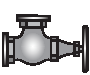
\includegraphics[scale=0.45]{../../figs/08HWEquivPipe/anglevalve} & Angle Valve & 150    \\
		\midrule
		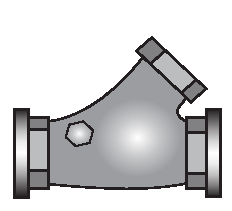
\includegraphics[scale=0.2]{../../figs/08HWEquivPipe/checkvalve}  & Check Valve & 100    \\
		\midrule
		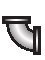
\includegraphics[scale=0.65]{../../figs/08HWEquivPipe/elbow}      & Elbow       & 50     \\
		\midrule
		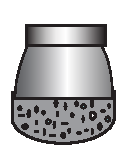
\includegraphics[scale=0.2]{../../figs/08HWEquivPipe/footvalve}   & Foot Valve  & 75     \\
		\midrule
		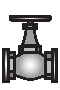
\includegraphics[scale=0.45]{../../figs/08HWEquivPipe/gatevalve}  & Gate Valve  & 35     \\
		\bottomrule
	\end{tabular}
\end{textblock*}


\begin{textblock*}{.35\textwidth}(13cm, 8cm)
	\centering
	
	\begin{tabular}{cccc}
		\toprule
		Pipe & Length (m) & diam (mm) & C   \\
		\midrule
		AB   & 10         & 500       & 125 \\
		\midrule
		BC   & 2000       & 275       & 150 \\
		\midrule
		BD   & 1500       & 250       & 100 \\
		\midrule
		DC   & 1000       & 300       & 100 \\
		\midrule
		CE   & 10         & 500       & 125 \\
		\bottomrule
	\end{tabular}
\end{textblock*}
%\begin{textblock*}{.6\textwidth}(2cm, 15cm)
%\cbox{
%\begin{itemize}
%\item[] Diam of equiv pipe for BDC (series) = 217.91 mm
%\item[] Diam of equiv pipe for BC (parallel) = 325.82 mm
%\item[] Diam of equiv pipe for AE (series) = 324.98 mm
%\item[] Q = 96.978 L/s
%\end{itemize}
%}
%\end{textblock*}
~
\vspace{13cm}

\cmini[0.9]{
	\textbf{Solution}
	\parb
	\cbox{
		
		The objective is to replace the system of five pipes $AB,\,BC,\,CD,\,DC$ and $CE$ with a single hydraulically equivalent
		pipe from $A$ to $E$. Then we can use the Hazen-Williams equation to find flow through the system.\parb
		Our process will be as follows:
		\begin{enumerate}
			\item Find the effective lengths of the pipes that have valves or fittings.
			\item Consider the series system of two pipes $BD$ and $DC$: find a hydraulically equivalent pipe $BDC$.
			\item Consider the parallel system of two pipes $BDC$ (just found above) and $BC$: find a hydraulically equivalent pipe $BC2$
			      for flow from $B$ to $C$.
			\item Consider the series system of three pipes $AB,\,BC2,\text{ and }CE$: find a hydraulically equivalent pipe $AE$.
			\item Use the General Energy Equation and the Hazen-Williams equation to find $Q$.
		\end{enumerate}
		
	}
}
\vfill
\cmini[0.9]{
	
	\cbox{
		\textbf{(1)} Find the effective lengths of the pipes that have valves or fittings.
		
		\begin{align*}
			L_{\text{eff}}     & = \text{Actual Length + Diameter}\times\left(\Sigma\frac{L_e}{D}\right) \\\\
			L_{\text{eff}(AB)} & = 10 + 0.5(75+50+100) = 122.5\,\text{m}                                 \\
			L_{\text{eff}(BC)} & = 2000 + 0.275(50+35+50) = 2037.1\,\text{m}                             \\
			L_{\text{eff}(BD)} & = 1500 + 0.250(150) = 1537.5\,\text{m}                                  \\
		\end{align*}
		
	}
	\parb
	\cbox{
		\textbf{(2)} Find a single equivalent pipe $BDC$ for the two pipes $BD$ and $DC$ in series.\parb
		
		Find the headloss between $B$ and $C$ for a flow of 100 L/s though $BD$ and $DC$, using the effective lengths of the pipes.
		
		\begin{align*}
			h_L        & = L\left(\frac{279000Q}{CD^{2.63}}\right)^{1.852}                                             \\\\
			h_{L(BD)}  & = 1537.5\left(\frac{279000\times 100}{100\times 250^{2.63}}\right)^{1.852} = 39.110\,\text{m} \\
			h_{L(DC)}  & = 1000\left(\frac{279000\times 100}{100\times 300^{2.63}}\right)^{1.852} = 10.467\,\text{m}   \\\\
			h_{L(BDC)} & = 39.110 + 10.467 = 49.577\,\text{m}                                                          \\
		\end{align*}
		
		\parb
		
		Find an equivalent pipe for $BDC$ (i.e., a pipe that has a head loss of 49.577 m for a flow of 100 L/s). We use an equivalent pipe with length 1000 m and resistance coefficient 100, and find the equivalent pipe diameter.
		
		\begin{align*}
			D       & = \left( \frac{279000Q}{C\left(\frac{h_L}{L}\right)^{0.54}}  \right)^{0.3802}                                      \\\\
			D_{BDC} & = \left( \frac{279000\times 100}{100\left(\frac{49.577}{1000}\right)^{0.54}}  \right)^{0.3802} = 217.92\,\text{mm} \\
		\end{align*}
		
	}
}
\cmini[0.9]{
	
	\cbox{
		\textbf{(3)} Now, consider pipe $BC$ and the pipe $BDC$ just found as a parallel system. Find an equivalent pipe for these two parallel pipes.\parb
		
		Assume a headloss of 10 m between $B$ and $C$ and find the flow through each of $BC$ and $BDC$:
		
		\begin{align*}
			Q                     & = \frac{CD^{2.63}\left(\frac{h_L}{L}\right)^{0.54}}{279000}                                      \\\\
			Q_{BC}                & = \frac{150\times 275^{2.63}\left(\frac{10}{2037.1}\right)^{0.54}}{279000} = 79.262\,\text{L/s}  \\
			Q_{BDC}               & = \frac{100\times 217.92^{2.63}\left(\frac{10}{1000}\right)^{0.54}}{279000} = 42.084\,\text{L/s} \\
			Q_{BC\text{ and }BDC} & = 79.262 + 42.084 = 121.35 \,\text{L/s}                                                          \\
		\end{align*}
		
		\parb
		
		A flow of 121.35 L/s between $B$ and $C$ through both pipes $BC$ and $BDC$ produce a headloss of 10 m. Find an equivalent pipe that replaces these two parallel pipes:
		
		\begin{align*}
			D_{BC\text{equiv}} & = \left( \frac{279000\times 121.35}{100\left(\frac{10}{1000}\right)^{0.54}}  \right)^{0.3802} = 325.83\,\text{mm} \\
		\end{align*}
		
	}
	
}

\cmini[0.9]{
	
	\cbox{
		\textbf{(4)} Now we have a series system: $AB,\, BC\text{equiv}$ and $CE$. Assume a flow of 100 L/s from $A$ to $E$, find the total headloss for this flow and then replace these three pipes with a single equivalent pipe.\parb
		
		\begin{align*}
			h_{L(AB)}             & = 122.5\left(\frac{279000\times 100}{125\times 500^{2.63}}\right)^{1.852} = 0.070450\,\text{m} \\
			h_{L(BC\text{equiv})} & = 1000\left(\frac{279000\times 100}{100\times 325.83^{2.63}}\right)^{1.852} = 7.0000\,\text{m} \\
			h_{L(CE)}             & = 10\left(\frac{279000\times 100}{125\times 500^{2.63}}\right)^{1.852} = 0.0057510\,\text{m}   \\\\
			h_{L(AE)}             & = 0.070450 + 7.0000 + 0.0057510 = 7.0762\,\text{m}                                             \\
		\end{align*}
		
		\parb
		
		Find the equivalent pipe that has a headloss of 7.0762 m for a flow of 100 L/s:
		
		\begin{align*}
			D_{AE} & = \left( \frac{279000\times 100}{100\left(\frac{7.0762}{1000}\right)^{0.54}}  \right)^{0.3802} = 324.99\,\text{mm} \\
		\end{align*}
	}
	
}

\cmini[0.9]{
	
	\cbox{
		\textbf{(5)} From the General Enery Equation (disregarding velocity head at $E$), headloss through the actual system is 6.7 m. We just need the flow that generates this headloss: \parb
		
		\begin{align*}
			Q_{AE} & = \frac{100\times 324.99^{2.63}\left(\frac{6.7}{1000}\right)^{0.54}}{279000} = 96.983\,\text{L/s} \\
		\end{align*}
		
		
	}
	
}




\end{document}
